\subsection{$b\rightarrow s\bar\mu\mu$}
\label{sec_bsmumu}
\begin{figure}[t]
 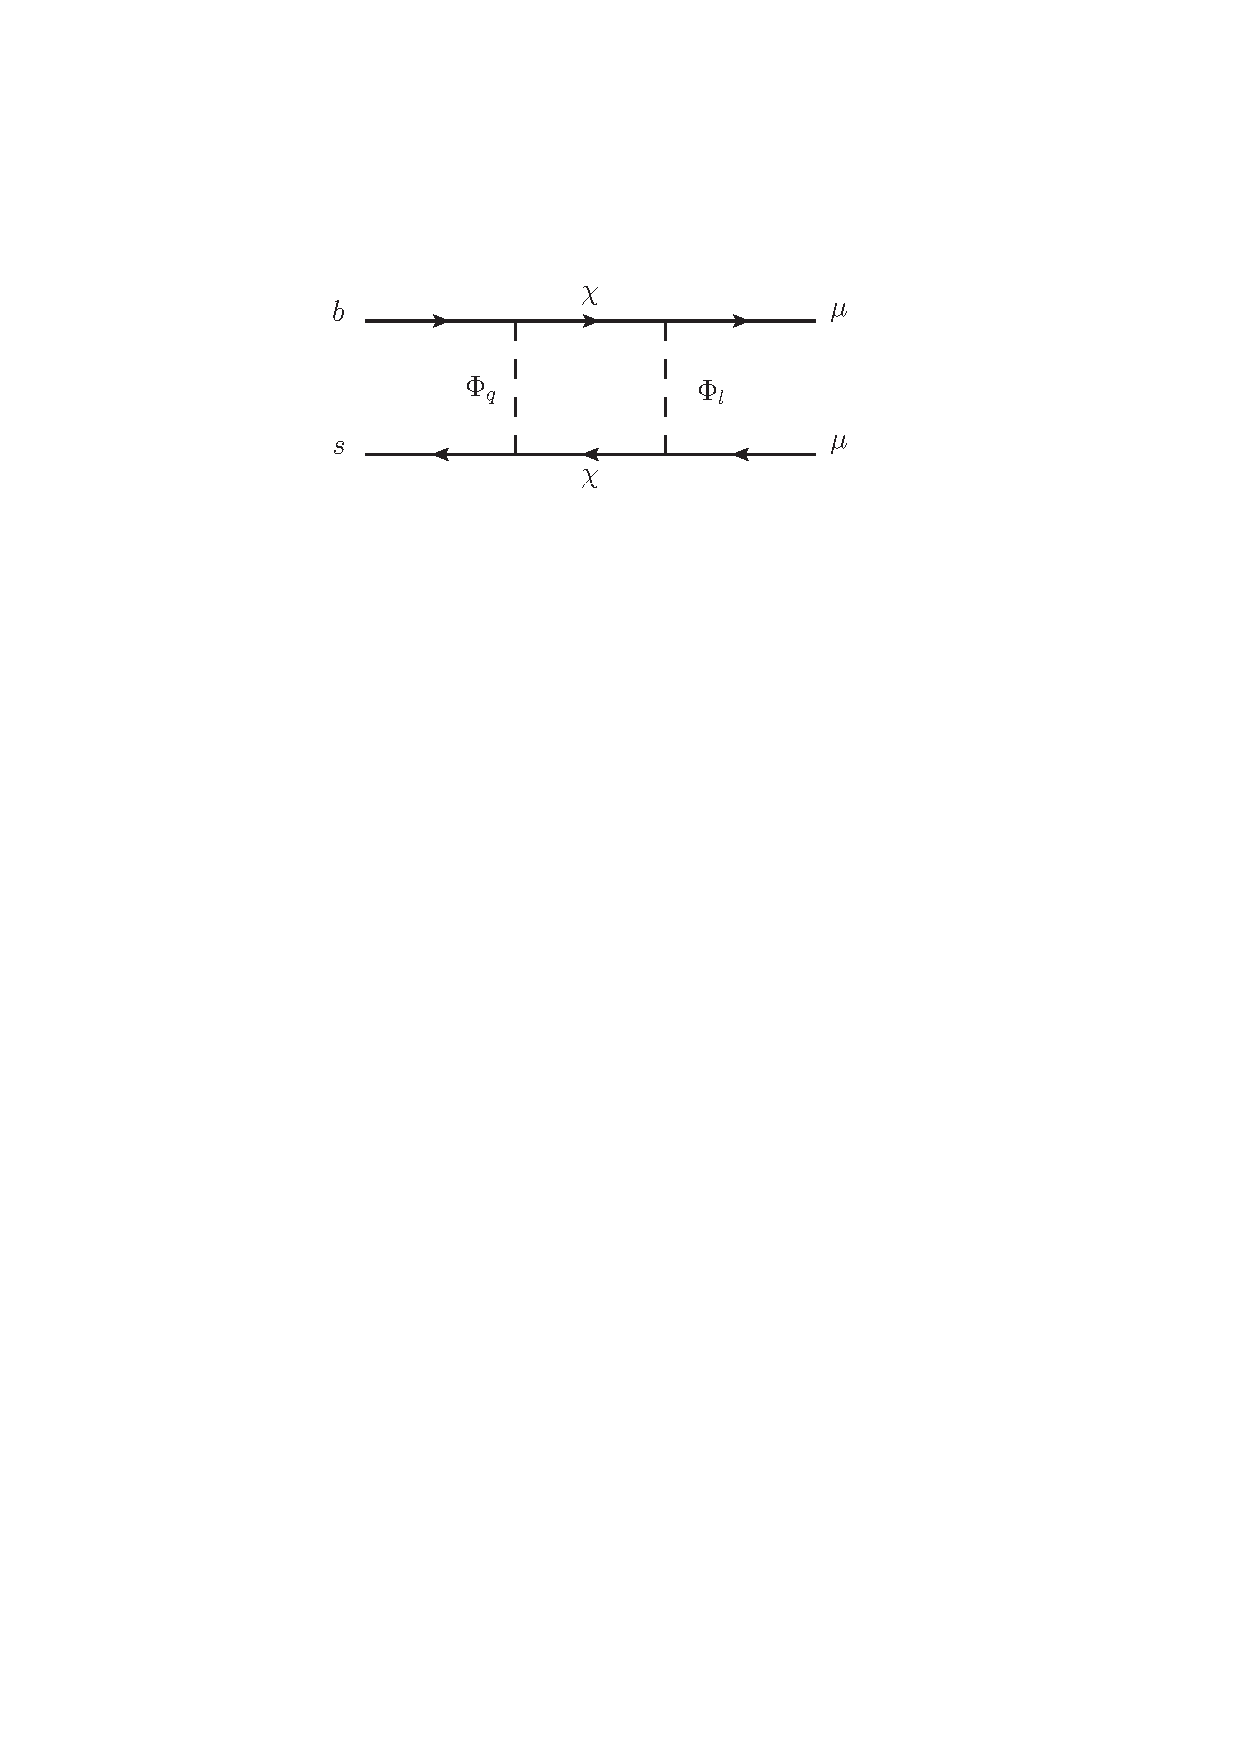
\includegraphics[width=1\textwidth]{../pics/bsmumu.pdf}
 \caption{Feynman diagrams for $b\rightarrow s \bar\mu\mu$ processes. In case of a Majorana particle being able to mediate such processes, crossed
 diagrams as (b) contribute (see text).}
 \label{pic_Bsmumu}
\end{figure}
Our first process targets anomalies in decays being induced by the quark level transition $b\rightarrow s\bar\mu\mu$. Our parameter set for this 
semileptonic process includes all our model parameters
\begin{align}
 \left(m, M_l, M_q, g_2^l\right).
\end{align}
Box diagrams of the kind as in picture \ref{pic_Bsmumu}a are usually not calculated 
all the way down to cross sections but one rather uses the formalism of effective field theory since the typical hadronic energy scale is of
$\mathcal{O}$(1 GeV) which is much lower than the weak scale $\mathcal{O}$(100 GeV) that is also the expected mass scale of our NP states. 
\\ \\ \noindent \textit{Matrix Element}\\
\noindent So we can use 
the OPE framework where they are integrated out and the external masses and momenta are set to zero. The amplitude in the full theory is
\begin{align}
 M =g_i^{q*} g_j^{q} g_m^{l*} g_n^l\int \frac{\dx^4 k}{(2\pi)^4} \frac{k^\rho}{D^\chi_k}\frac{1}{D^q_k} \frac{1}{D^l_k} \frac{k^\sigma}{D^\chi_k} \left(\bar L_L^n \gamma_\rho Q_L^j\right) \left(\bar Q_L^i \gamma_\sigma L_L^m\right)
 \label{eq_matElemBSmumu}
\end{align}
with $k$ as the internal momentum and the denominators of the respective particle $a$ with momentum $k$ $D^a_k = k^2-M_a^2$ and the $\ti\epsilon$ terms in the denominators are already omitted
due to Wick-rotation later on when the integral is performed. The reasons why $m$ in the fermion propagators is missing
and why there is a Lorentz structure in the couplings, are connected. Since we have a model which couples only to left handed particles $\psi_L = P_L \psi$,
the fermion currents look like $\bar \psi_L (\slashed{k}+m)\varphi_L = \bar \psi P_R (k^\mu \gamma_\mu+m) P_L\varphi$. Further
$\{P_{L,R},\gamma^\mu\} = \gamma^\mu P_{R,L}$, $P_{L,R}^2 = P_{L,R}$ and $P_R P_L = 0$, so we are left over with the four fermion expression in 
\eqref{eq_matElemBSmumu}. We can also reexpress $k^\rho k^\sigma = k^2 g^{\rho\sigma}/4$ under the integral. This results from spherical coordinates where
every combination $\rho\neq\sigma$ would include at least one uneven angular function. When the spherical integral is performed, they would lead to zero. The 
4 in the denominator is the spacetime dimension. The spherical integral $\dx \Omega$ itself just gives a $2\pi^2$ and we are left with the momentum integral
which is not problematic since it does not diverge
\begin{align}
 M \propto \frac{1}{32\pi^2} \int\limits_0^\infty \dx k \frac{k^5}{{D^\chi_k}^2D^l_k D^q_k} = \frac{K(x_q,x_l)}{64\pi^2 m_\chi^2}
\end{align}
with
\begin{align}
 K(x,y) &= \frac{K(x)-K(y)}{x-y} > 0, \qquad\forall x,y > 0\\
 K(x)&=\frac{1-x+x^2\log(x)}{(x-1)^2} \stackrel{x\rightarrow 1}{=} \frac32.
\end{align}
In the SM, the fermion currents do not combine quarks and leptons. To compare the NP contribution to this process, we have to rearrange the fermion currents,
so that we have the same structure. This will be done by the Fierz identities.
\\ \\ \noindent \textit{Fierz Identities}\\
They usually relate a Dirac quadrilinear, containing four spinors, with a sum of rearranged Dirac quadrilinears \cite{Fierz}
\begin{align}
  \left[\bar w_1\Gamma_I^{} w_2\right] \left[\bar w_3 \Gamma^I w_4 \right] =: e_I(1234) = \sum\limits_J K_{IJ} e_J(1432)
\end{align}
with an (anti)spinor $w$ and $\Gamma_I$ as a set of Dirac matrices whereby $I=S,V,T,A,P$ representing $I,\gamma^\mu,\sigma^{\mu\nu},\gamma^\mu\gamma_5,\gamma_5$, 
respectively. The coefficients $K_{IJ}$ are real numbers and can differ for other arrangements.
% \begin{align}
%  F_{IJ}=\frac14\begin{pmatrix}
%     1&1&\frac12&-1&1\\
%     4&-2&0&-2&-4\\
%     12&0&-2&0&12\\
%     -4&-2&0&-2&4\\
%     1&-1&\frac12&1&1\\
%  \end{pmatrix}_{IJ}.
% \end{align}
\noindent For our purpose we want to transform the quadrilinear in \eqref{eq_matElemBSmumu}. By expanding there are four terms
\begin{align}
 e_V(1234)+e_A(1234)-\left(e'_V(1234) + e'_A(1234)\right).
 \label{eq_fierz}
\end{align}
The primed quadrilinears represent a pseudoscalar combination of two parity partners, e.g. $e'_V = \left[\bar w\gamma^\mu w\right]\left[w\gamma_\mu\gamma_5w\right]$
which are transformed with $F^\text{T}$. We can see that \eqref{eq_fierz} is an invariant for every order and so we can simply rearrange the quadrilinear.
\\ \noindent For later cases \eqref{eq_crossedBox} we also point out that 
\begin{subequations}
\begin{align}
 \left[\bar w_1 P_R w_2\right]\left[\bar w_3 P_L w_4\right] =& \frac12  \left[\bar w_3 \gamma_\mu P_L w_2\right]\left[\bar w^c_4 \gamma^\mu P_L w_1^c\right]\\
 =& \frac12  \left[\bar w_3 \gamma_\mu P_L w_2\right]\left[\bar w_1 \gamma^\mu P_L w_4\right].
 \label{eq_fierzSPtoVA}
\end{align} 
\end{subequations}

 \noindent \textit{Additional $SU(2)_L$-invariant term}\\
\noindent The operator $O_\delta=\left(\bar Q_L^i \gamma_\rho Q_L^j\right)\left(\bar L_L^m \gamma^\rho L_L^n\right)$ is not the only one which is a singlet
in the isospin space but $O_\tau=\left(\bar Q_L^i\vec \tau \gamma_\rho Q_L^j\right)\left(\bar L_L^m\vec \tau \gamma^\rho L_L^n\right)$ as well which enables
charged currents. The eventual operator is a superposition of these two. There might be several ways of computing the model dependent, relative 
prefactor $\xi$ of $O_\tau$  but one possibility is to regard the particles at each vertex as isospin multiplets. Since we want the vertices to be 
$SU(2)_L$-invariant, we 
decompose the product and focus on the singlet. This will be done for all four vertices per diagram which are multiplied and then added up for every diagram,
one can write down using these operators. For model A, this calculus can be done equivalently but can be skipped, because no charged currents as 
$b \bar u \rightarrow \mu \bar \nu$ are not induced, thus the prefactor of $O_\tau$ has to be zero and therefore 
\begin{align}
  \mathcal{L}^{\textbf{1}}_\text{eff} \supset \frac{K(x_q,x_l)}{m_\chi^2}\frac{g_i^{q*} g_j^{q*} g_m^l g_n^l}{64\pi^2} \times O_\delta.
 \label{eq_LagBSmumuModA}
\end{align}
In the case of higher dimensional isospin multiplets, processes of the just mentioned kind occur and thus we have three distinct types, with respect to 
their prefactor that can be checked by expanding $O_\delta + \xi O_\tau$, namely $\bar d d\rightarrow \bar l l$, $\bar d d \rightarrow \bar\nu \nu$ and 
$d \bar u\rightarrow l\bar\nu$. \\
\noindent To get the singlet expression we can make use of the Clebsch-Gordan coefficients, known from spin arithmetics which also obey an $SU(2)$-Group.
They can be read off the tables from (PDG). For a triplet ($\chi$) and two doublets ($\Phi$ and $D=Q,L$) we get
\begin{align}
 \frac{1}{\sqrt{3}}\left(\chi_3\Phi_1D_1 - \frac{1}{\sqrt{2}}\chi_2\left(\Phi_2D_1+\Phi_1 D_2\right) + \chi_1\Phi_2D_2 \right).
 \label{eq_CG}
\end{align}
The indices represent the components of the respective multiplets. One has to be careful which vertex one is looking at while using \eqref{eq_CG} in reference
to the Lagrangian \eqref{eq_modelLagrangian}. An incoming $u$-quark occupies the first isospin component in the quark doublet $Q$ but an outgoing one the 
second of $\bar Q$. Keeping this in mind we can look at each vertex of figure \ref{pic_Bsmumu} and examine the applicable coefficient. This is examplarily
depicted in figure \ref{pic_CG} for a generic $\bar d d\rightarrow \bar l l$ process that also represents $ b  \rightarrow s\bar \mu \mu$.
\begin{figure}[t]
 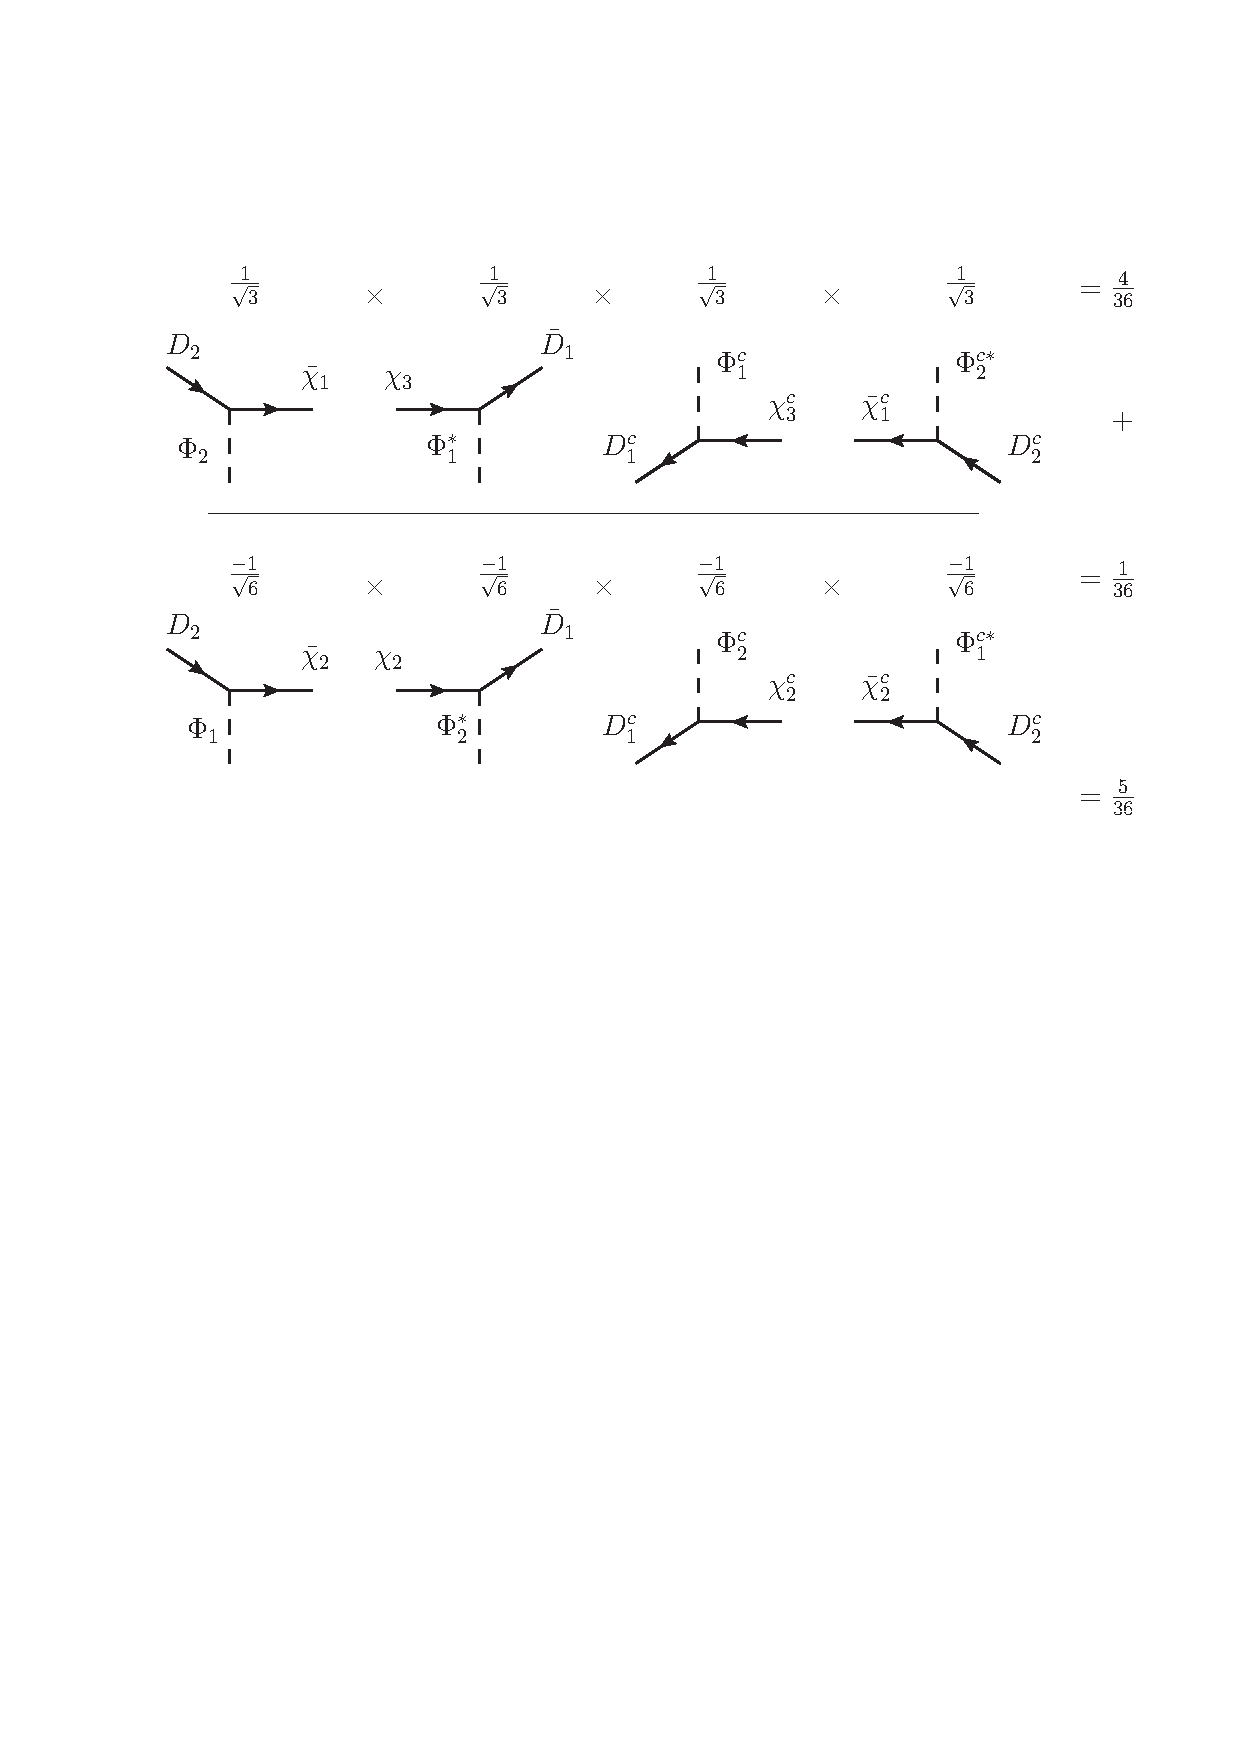
\includegraphics[width=\textwidth]{../pics/CG.pdf}
 \caption{$SU(2)_L$ singlet representation at each vertex of figure \ref{pic_Bsmumu} with the respective Clebsch-Gordan coefficients from \eqref{eq_CG}. 
 This is exemplary for $\bar d d\rightarrow \bar d d$ processes which get contributions from two different particle configurations.}
 \label{pic_CG}
\end{figure}
This gives an overall factor of $\sfrac{5}{36}$. The computation for the remaining two types is similar and yields $\sfrac{4}{36}$ for 
$\bar d d\rightarrow \bar \bar \nu \nu$ and $\sfrac{1}{36}$ for $\bar u d \rightarrow \bar \nu l$. With these three fractions, multiplied by a 
phenomenological constant $\eta=4\cdot R_\chi$ (coming from four vertices for the box diagram and $R_\chi$ is the dimension of the $\chi$ multiplet) 
and the respective relations from $O_\delta + \xi O_\tau$ for each type 
we can extract the prefactor $\xi=\sfrac23$. Finally, we can write down the effective Lagrangian for the triplet case
\begin{align}
 \mathcal{L}^{\textbf{3}}_\text{eff} \supset \frac{K(x_q,x_l)}{m_\chi^2}\frac{g_i^{q*} g_j^{q*} g_m^l g_n^l}{64\pi^2}\times\left(O_\delta + \frac23 O_\tau\right).
 \label{eq_LagBSmumuModB}
\end{align}
\\ \textit{Crossed Boxes}\\
\noindent As we assume our DM candidate $\chi^0$ to be Majorana, there are also contributions from crossed boxes (fig. \ref{pic_Bsmumu}b) for uncharged
currents like our process of interest $\bar d d\rightarrow \bar l l$. Compared to the former matrix element \eqref{eq_matElemBSmumu} we have some changes
for the crossed box diagram \cite{1411.6743}. Using the Feynman rules for internal Majorana particles \eqref{eq_majoProp} and the action of $C$ \eqref{eq_ChargeConj}, 
we see that now the masses in the fermion propagators remain. The momentum integral similarly to the pure Dirac case yields
\begin{align}
 M_\text{box} \propto \int\limits_0^\infty \dx k \frac{k^3 \cdot m_\chi^2}{{D^\chi_k}^2D^l_k D^q_k} = \frac{G(x_q,x_l)}{2m_\chi^2}
 \label{eq_crossedBox}
\end{align}
with similar (but not identical) loop functions
\begin{align}
 G(x,y) &= \frac{G(x)-G(y)}{x-y} < 0,\qquad \forall\, x,y>0\\
 G(x)&=\frac{1-x+x\log(x)}{(x-1)^2} \stackrel{x\rightarrow 1}{=} \frac12.
\end{align}
Concerning the $SU(2)_L$ invariance, the crossed box can just have the uncharged particle state for the internal lines. Therefore one gets only $\sfrac{1}{36}$
which is one fifth of the bare Dirac contribution. The two terms with $K(x_q,x_l)$ and $G(x_q,x_l)$, respectively, have opposite signs so that they can cancel
each other out and hence may reduce the impact of constraints from observables.\\
\\ \textit{New Physics Contribution}\\
\noindent Now we will gather up the information to get another bound for our model. There are two operators in the effective Hamiltonian for $b\rightarrow s\mu\mu$
transitions, $O_9$ and $O_{10}$ (sec. \ref{sec_flAnom}). The expression for the Wilson coefficient $C_9 = -C_{10}$ \cite{1408.1627} is obtained by comparing the 
coefficients from the 4-fermi operator in the effective Lagrangians and the effective Hamiltonian
\begin{align}
 C_9^{\textbf{1}} &= N \frac{g_2^{q*}g_3^q|g_2^l|^2}{m^2} \frac{1}{128\pi^2} \left(K(x_q,x_l) + G(x_q,x_l)\right)\\
 C_9^{\textbf{3}} &= N \frac{g_2^{q*}g_3^q|g_2^l|^2}{m^2} \frac{5}{384\pi^2} \left(K(x_q,x_l) + \frac15 G(x_q,x_l)\right)
 \label{eq_WilsonBsmumu}
\end{align}
with
\begin{align}
 N = \left(\frac{4G_F}{\sqrt{2}} V_{ts}^*V_{tb} \frac{\alpha_\text{EM}}{4\pi}\right)^{-1}.
\end{align}
With the formulae given here, one could also examine anomalies in other semileptonic decays, i.e. $b \rightarrow s\nu\nu$ \cite{1409.4557} or $B \rightarrow D\tau\nu$ \cite{1507.03233}. 
It is difficult to explain the latter at least with this kind of model, where these processes emerge at loop level and have to compete with the 
SM effect, which is at tree-level. The former can give bounds in general but since you cannot distinguish different neutrino flavours experimentally.
and we are only coupling to muonic ones, the contribution is even lower. In the triplet case \eqref{eq_LagBSmumuModB} the prefactors just calculated 
of the kind $\bar dd\rightarrow \bar\nu\nu$
are also small compared to the other ones enabling an even larger parameter space. So we expect $b\rightarrow s\bar \mu \mu$ among the semileptonic
processes to give the strongest constraints.
 

% Prefactors for other representations are listed in table below.

% \begin{table}[h]
% \begin{tabular}{c|cccc}
%  $(\chi,\Phi)$& (1,2) & (3,2) & (4,3) & (5,4)\\
%  \hline
%  $X$ & $0$ & $\sfrac23$ & $\sfrac59$ & $\sfrac12$
%  \end{tabular}
%  
% \end{table}
